\section{Homepage}

\subsection{General description}
The homepage analysis of \url{https://www.siciliangoodness.com/} is performed with many screens since it is developed vertically.

	\begin{figure}[H]
	\centering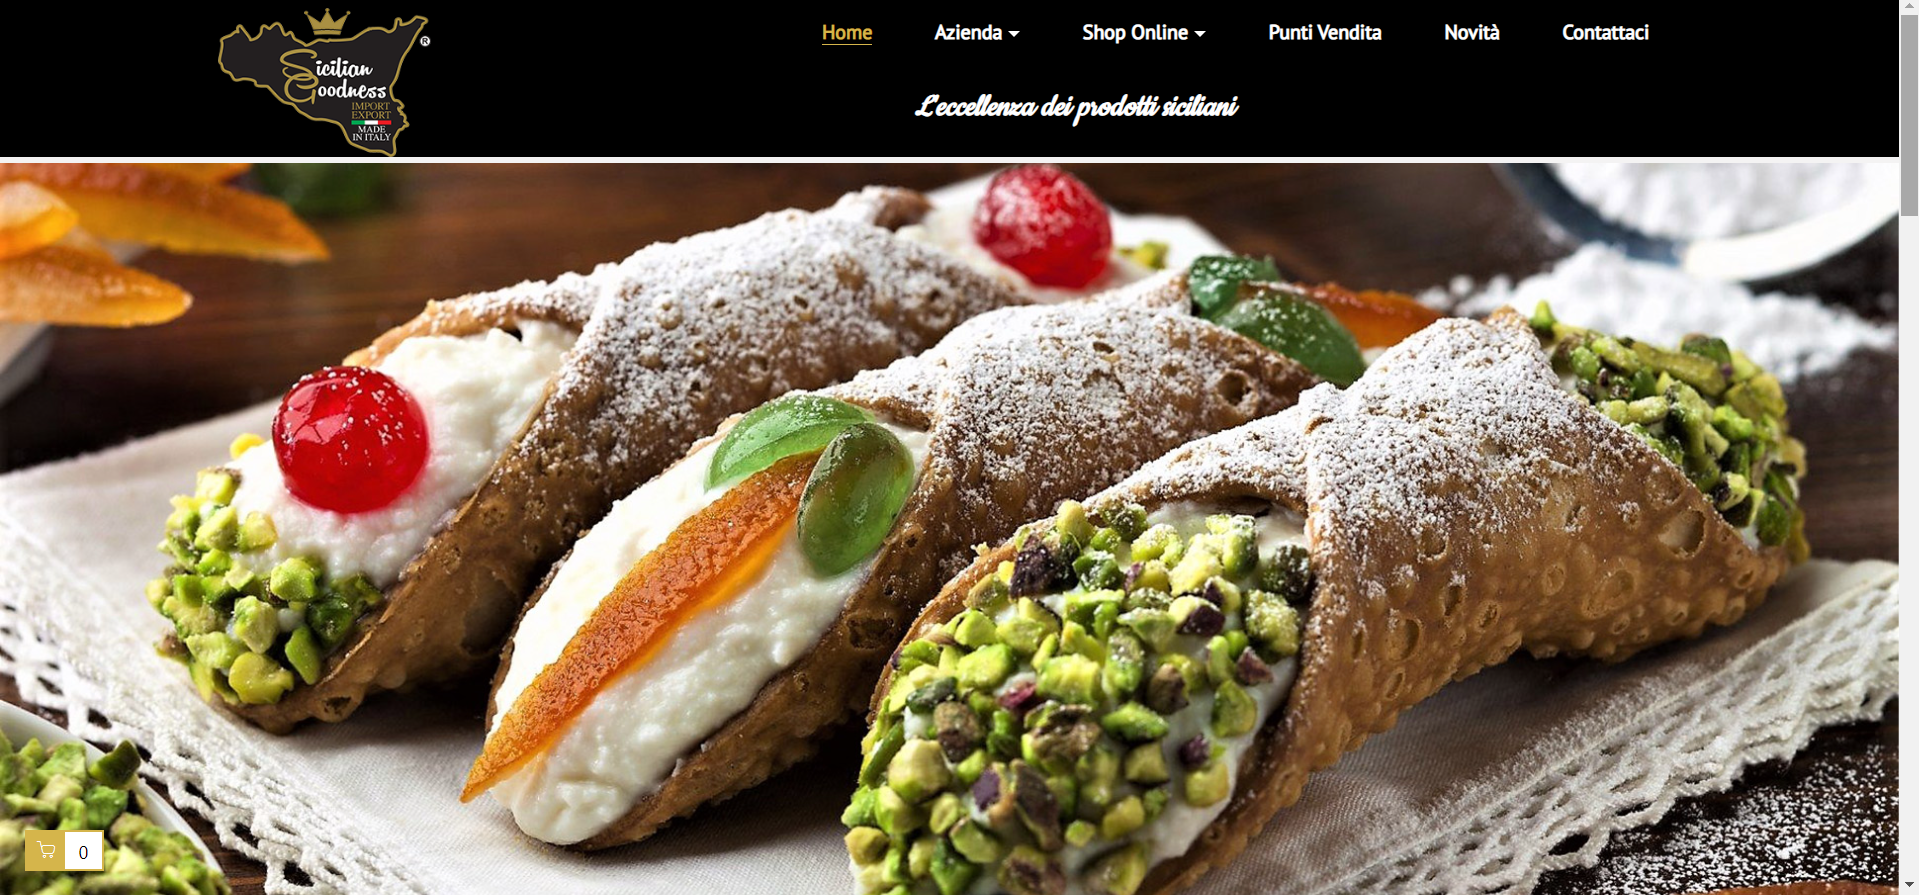
\includegraphics[width=12cm]{Img/hom1.png}
	\caption{Homepage 1}
	\end{figure}

In the most important part of the homepage, visible without scrolling, you can see some important and recurring elements on websites, such as:

\begin{itemize}
	\item the logo is well-suited in the top-left corner;
	\item the breadcrumb for the navigation;
	\item the colors are used well (white and black, readable).
\end{itemize}

As we can see in the images below we have a problem with the images of the homepage which are constantly changing. 
Even if today this is a common practice, the changing of the images can confuse the average user.
Especially in the \textbf{\hyperlink{hom5}{Figure 6}}, the products seem to be clickable but they are not, so the visual metaphore is not respected. \newline

\begin{figure}[H]
	\centering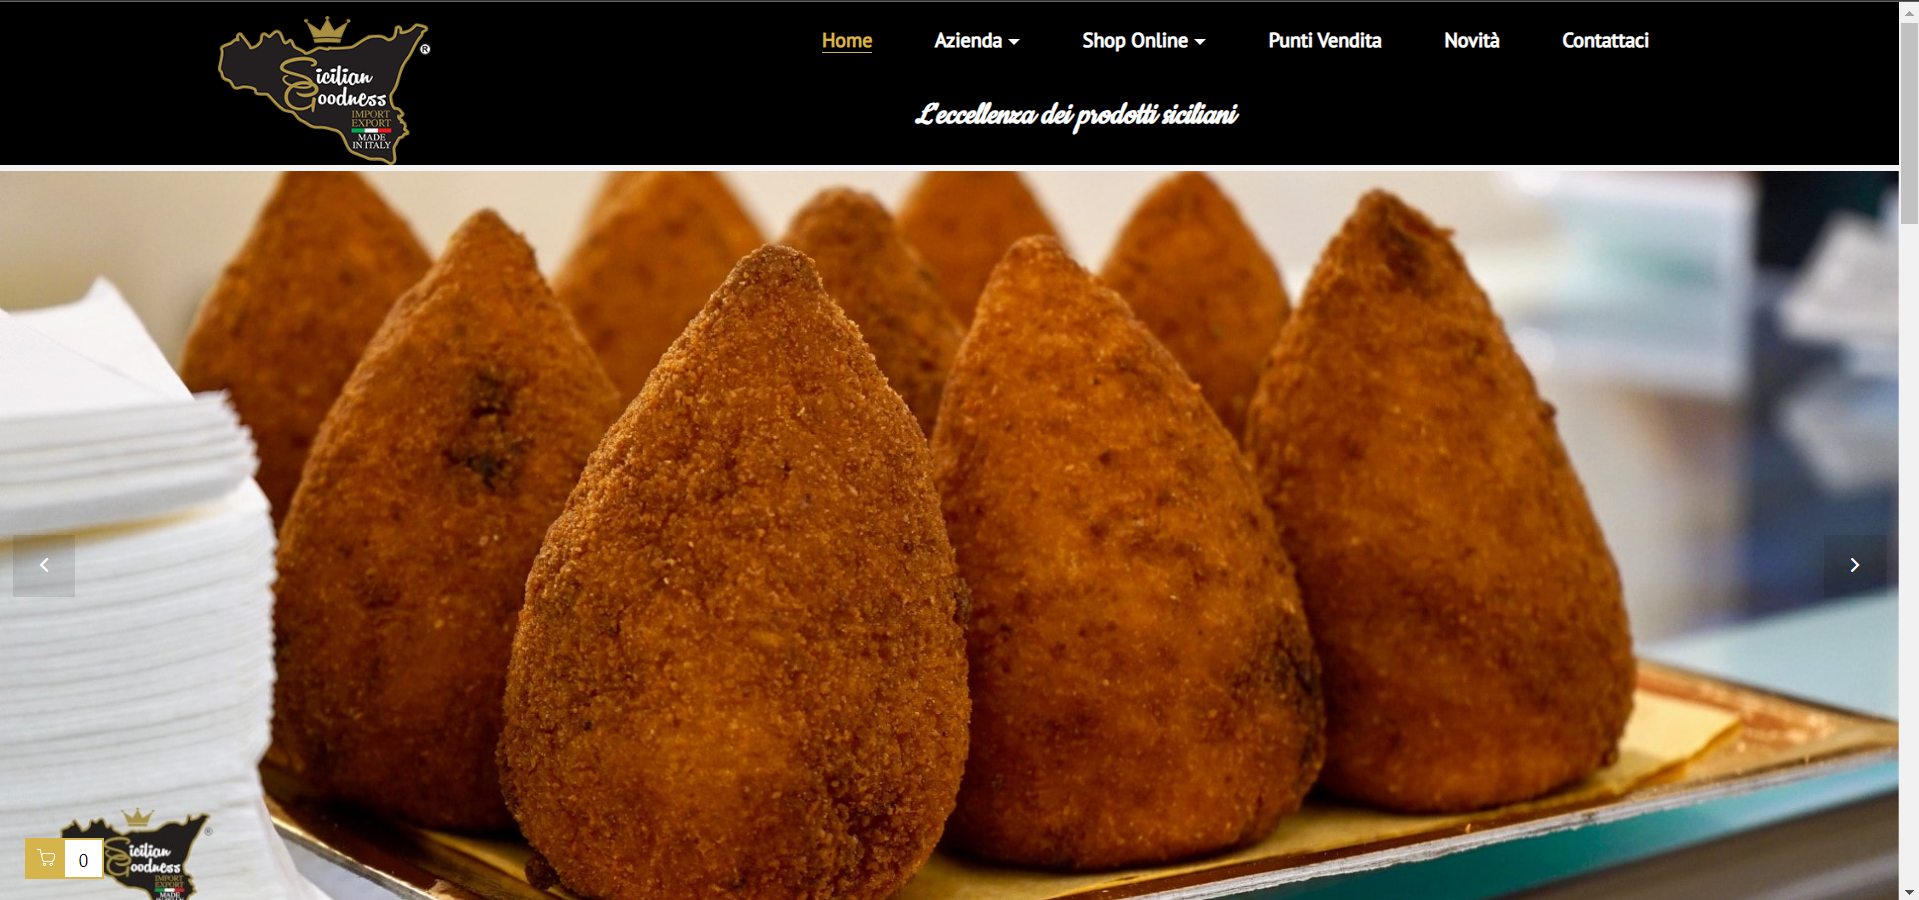
\includegraphics[width=12cm]{Img/hom2.png}
	\caption{Homepage 2}
\end{figure}

\begin{figure}[H]
	\centering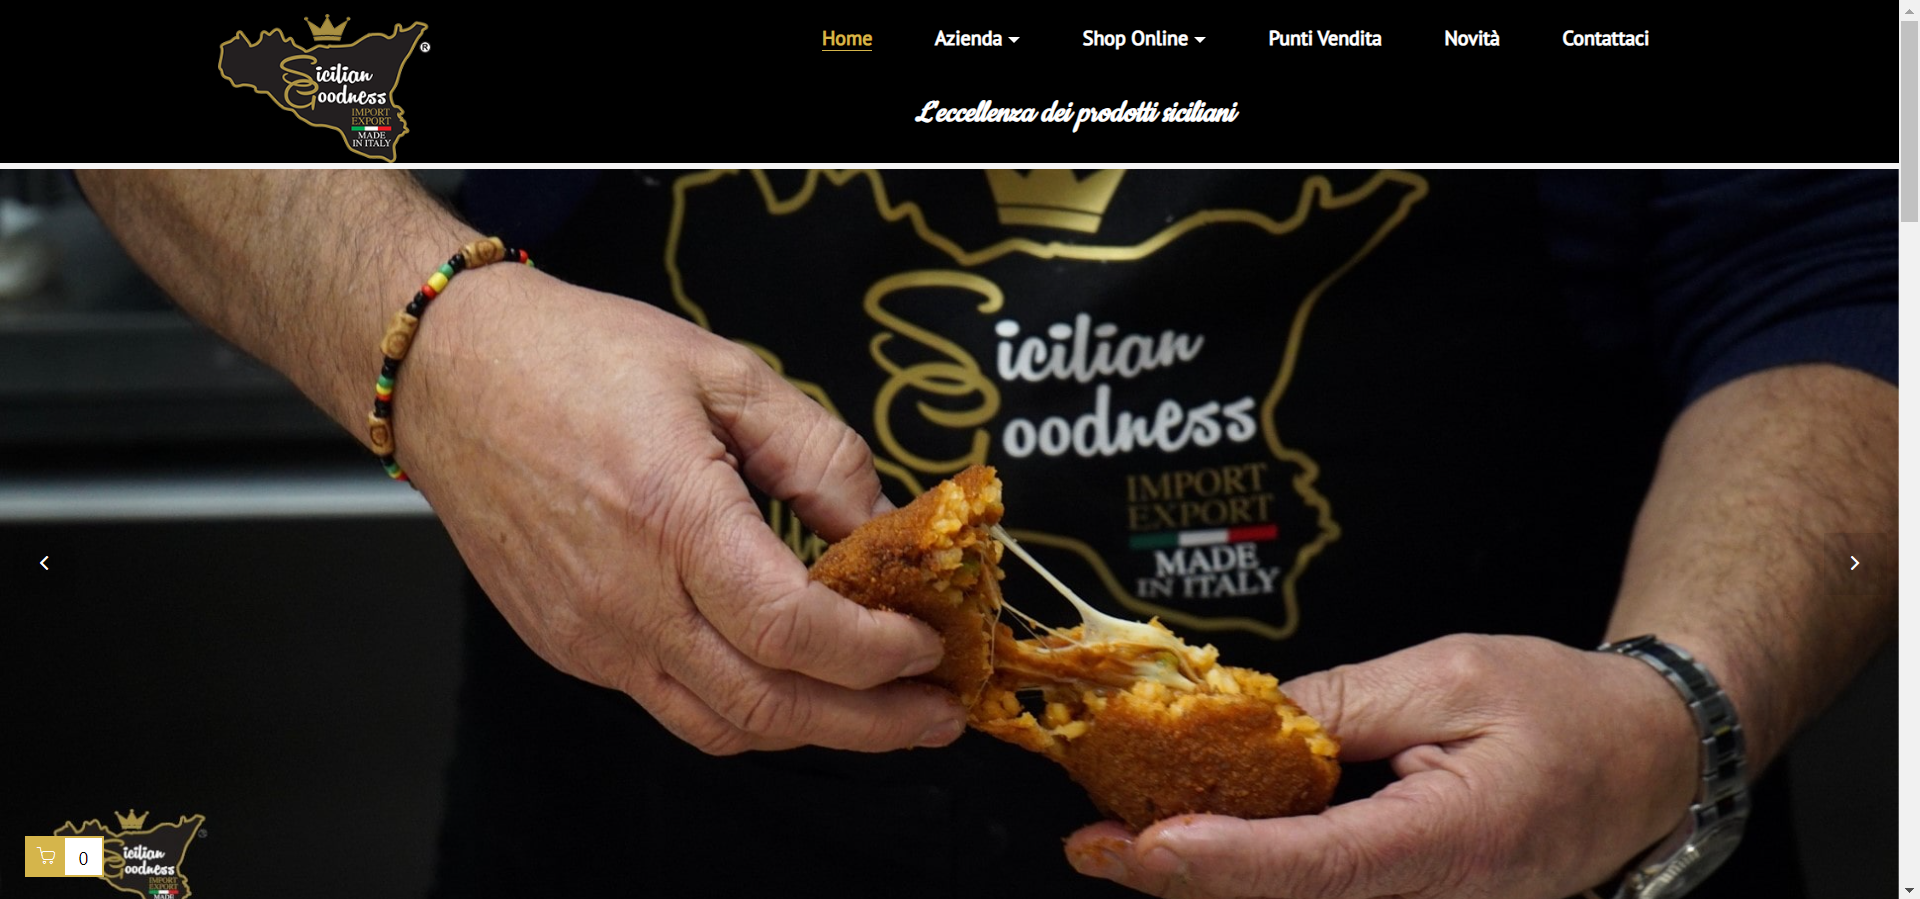
\includegraphics[width=12cm]{Img/hom3.png}
	\caption{Homepage 3}
\end{figure}

\begin{figure}[H]
	\centering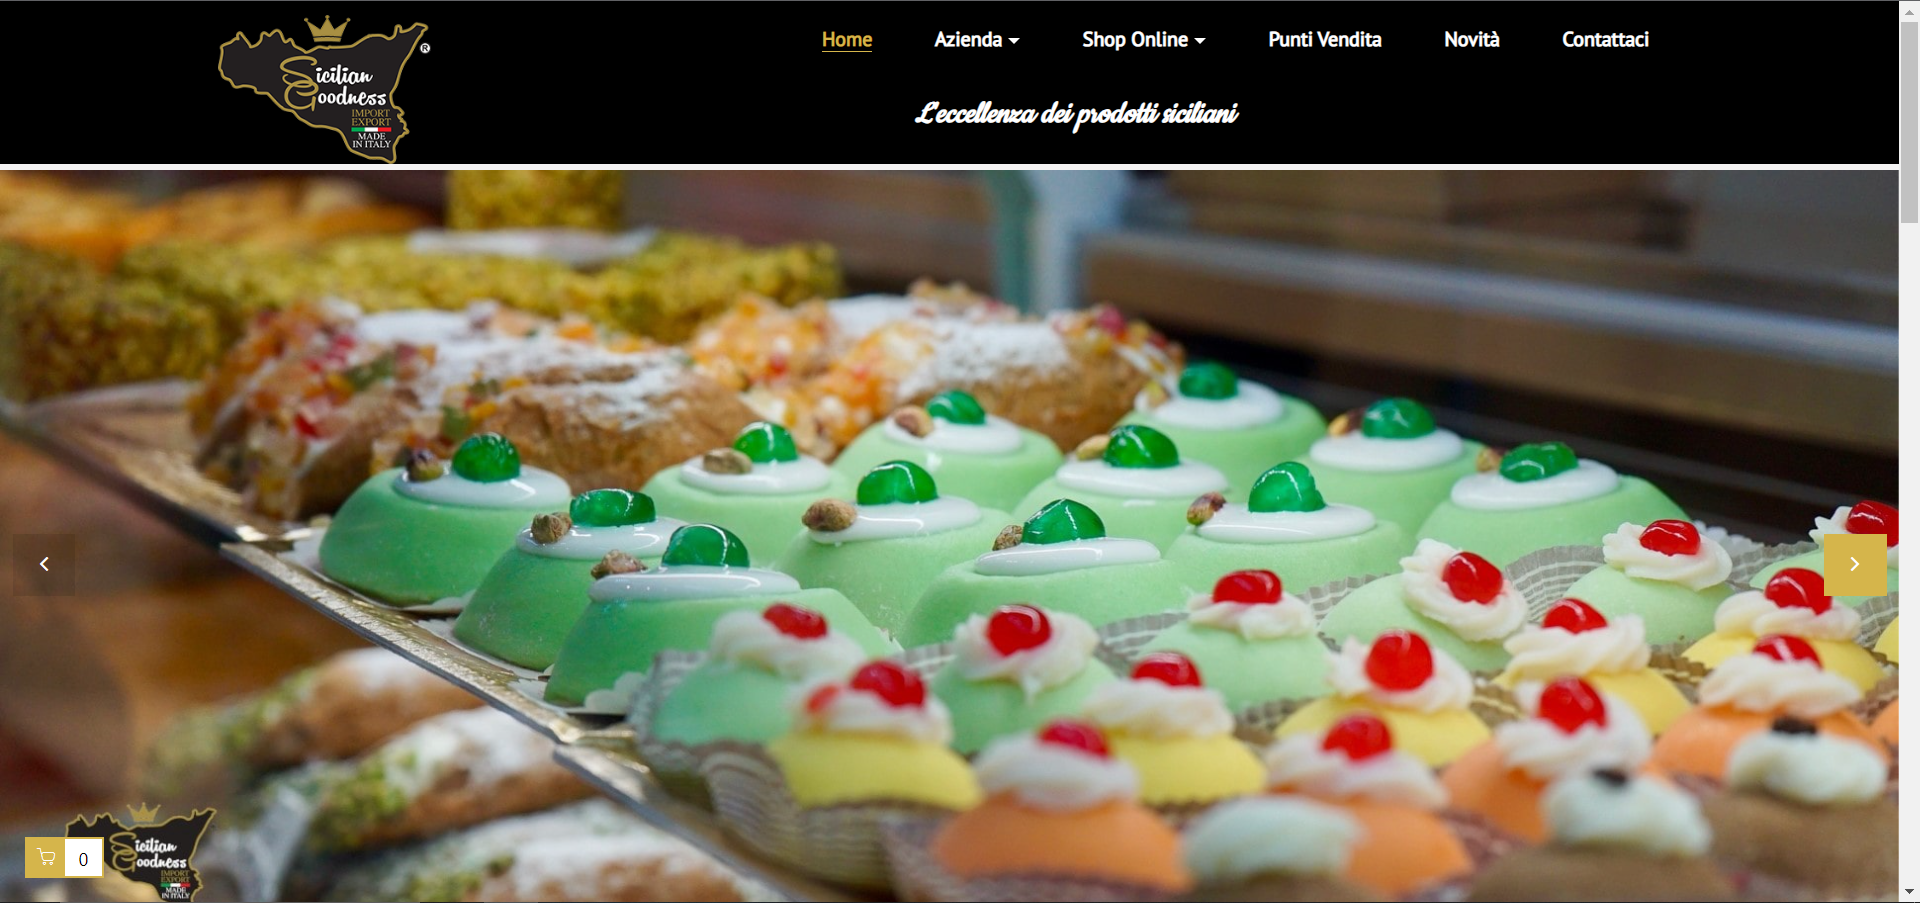
\includegraphics[width=12cm]{Img/hom4.png}
	\caption{Homepage 4}
\end{figure}

\begin{figure}[H]
	\label{hom5}
	\centering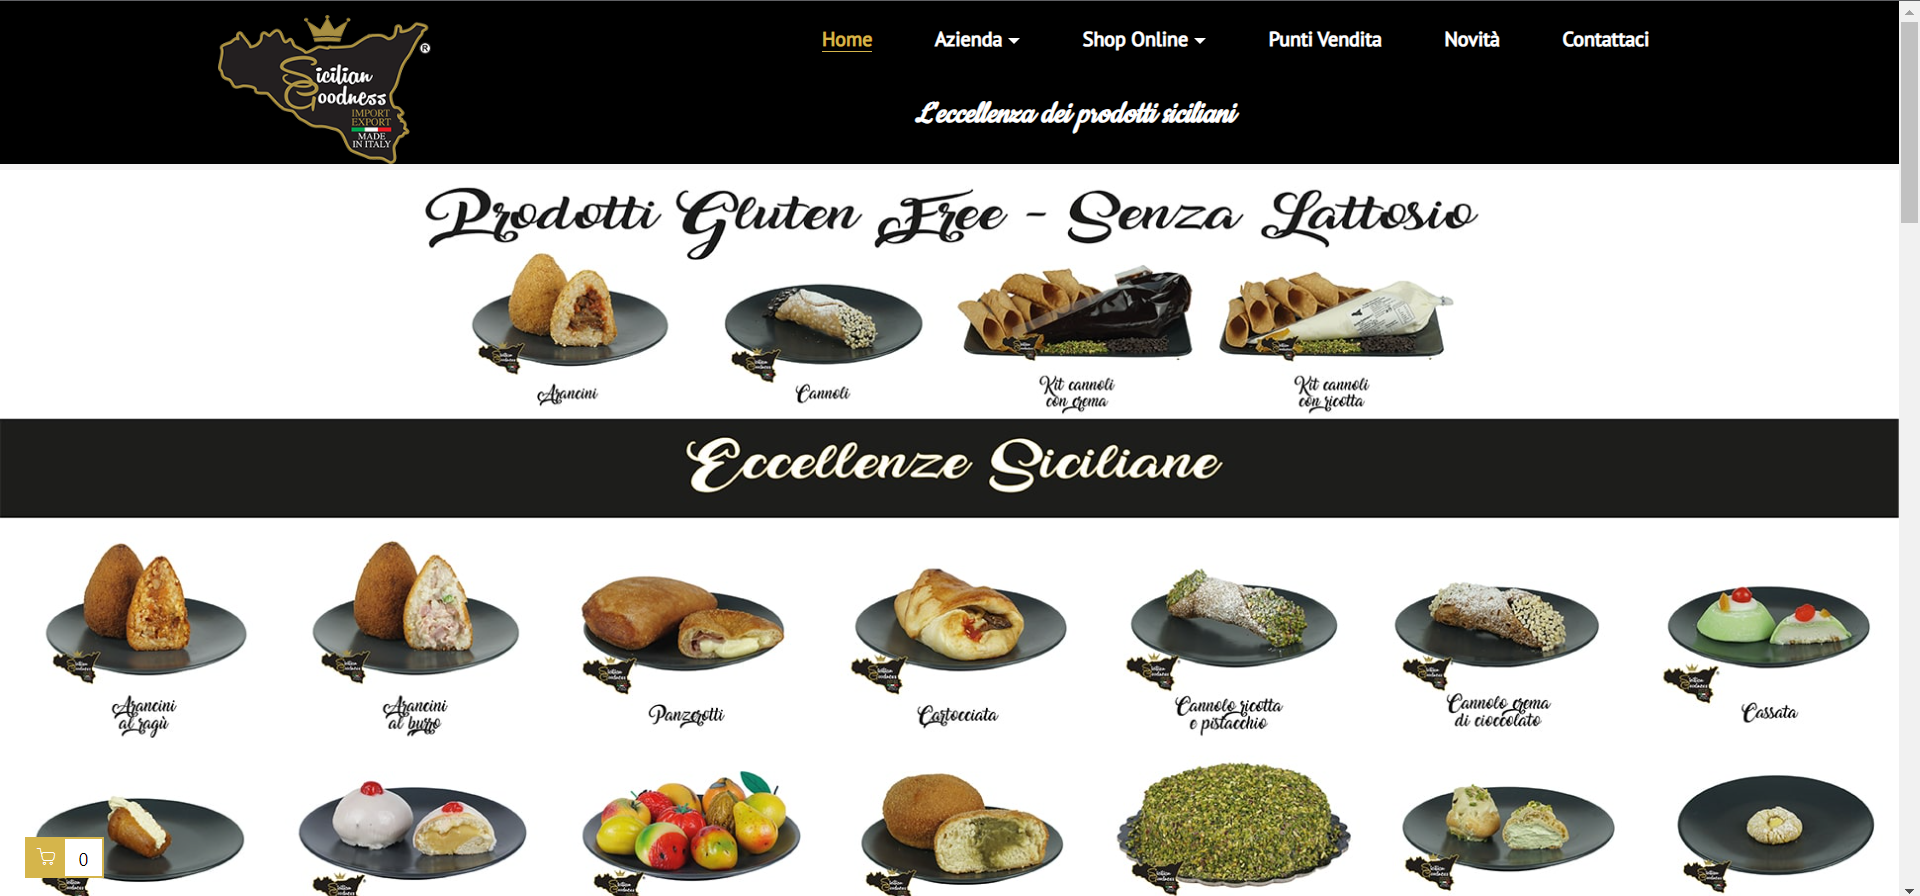
\includegraphics[width=12cm]{Img/hom5.png}
	\caption{Homepage 5}
\end{figure}

\pagebreak

As we can see in the next two pictures, in the following two scrolls we have the content of the page.

\begin{figure}[H]
	\centering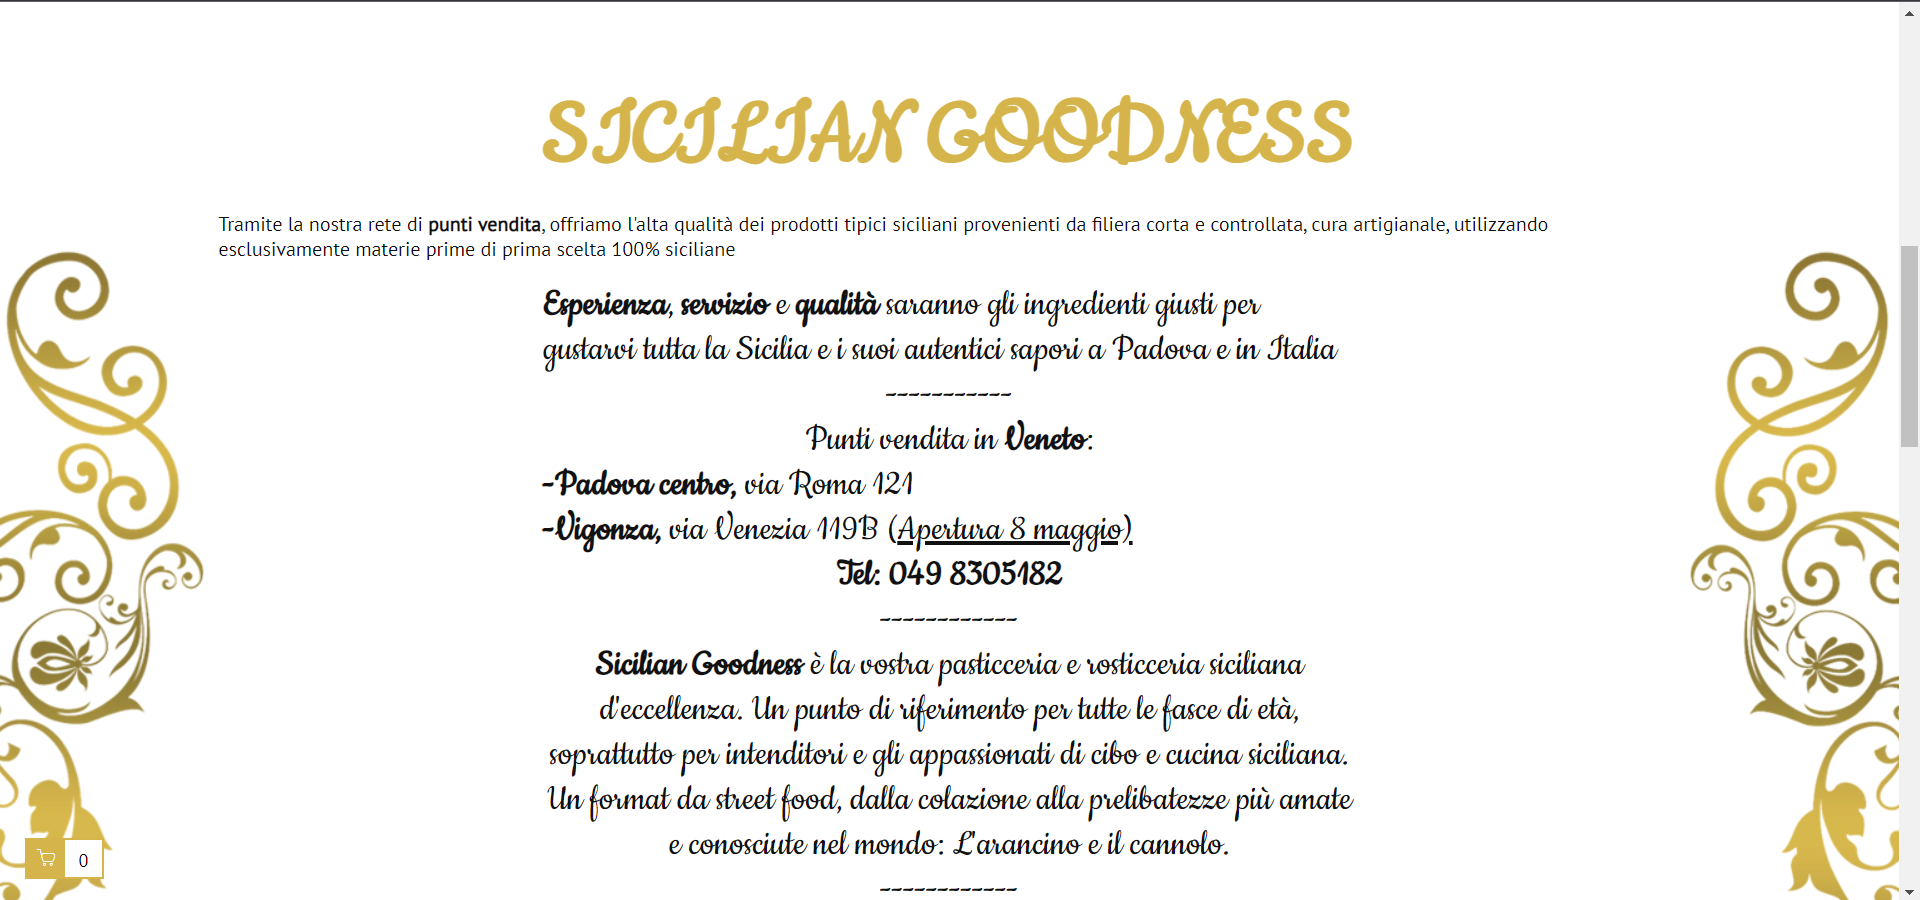
\includegraphics[width=12cm]{Img/content1.png}
	\caption{Content 1}
\end{figure}

\begin{figure}[H]
	\centering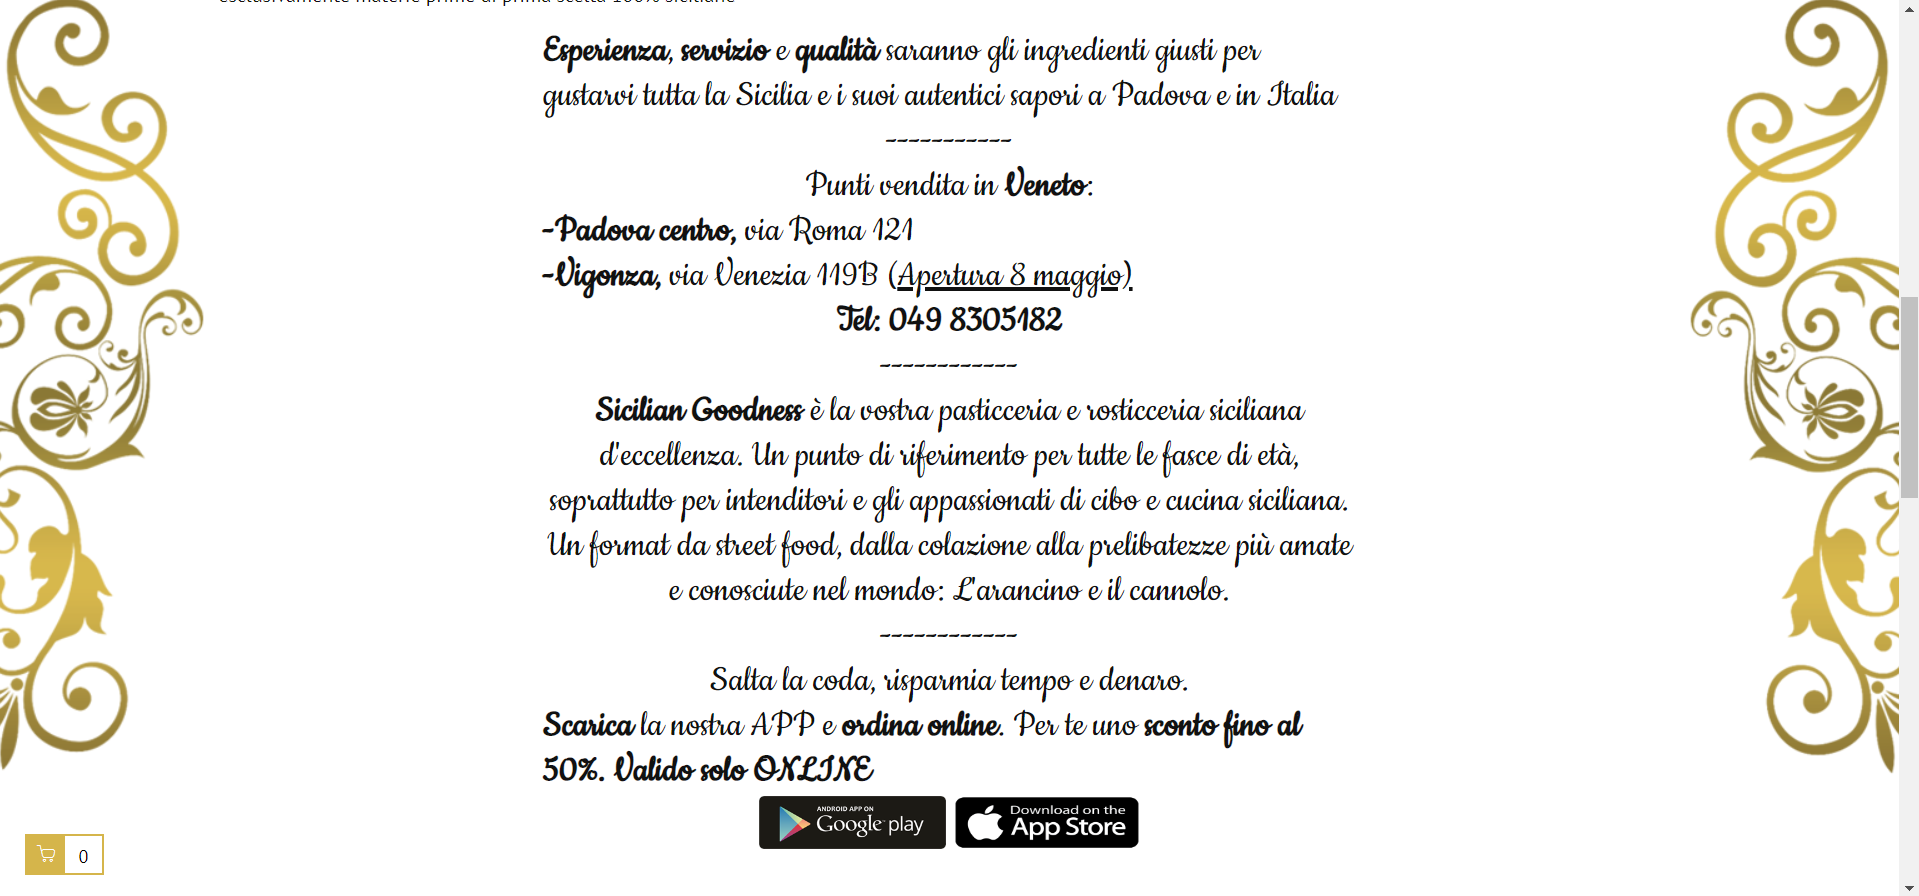
\includegraphics[width=12cm]{Img/content2.png}
	\caption{Content 2}
\end{figure}

The footer include all the information about the company.

\begin{figure}[H]
	\centering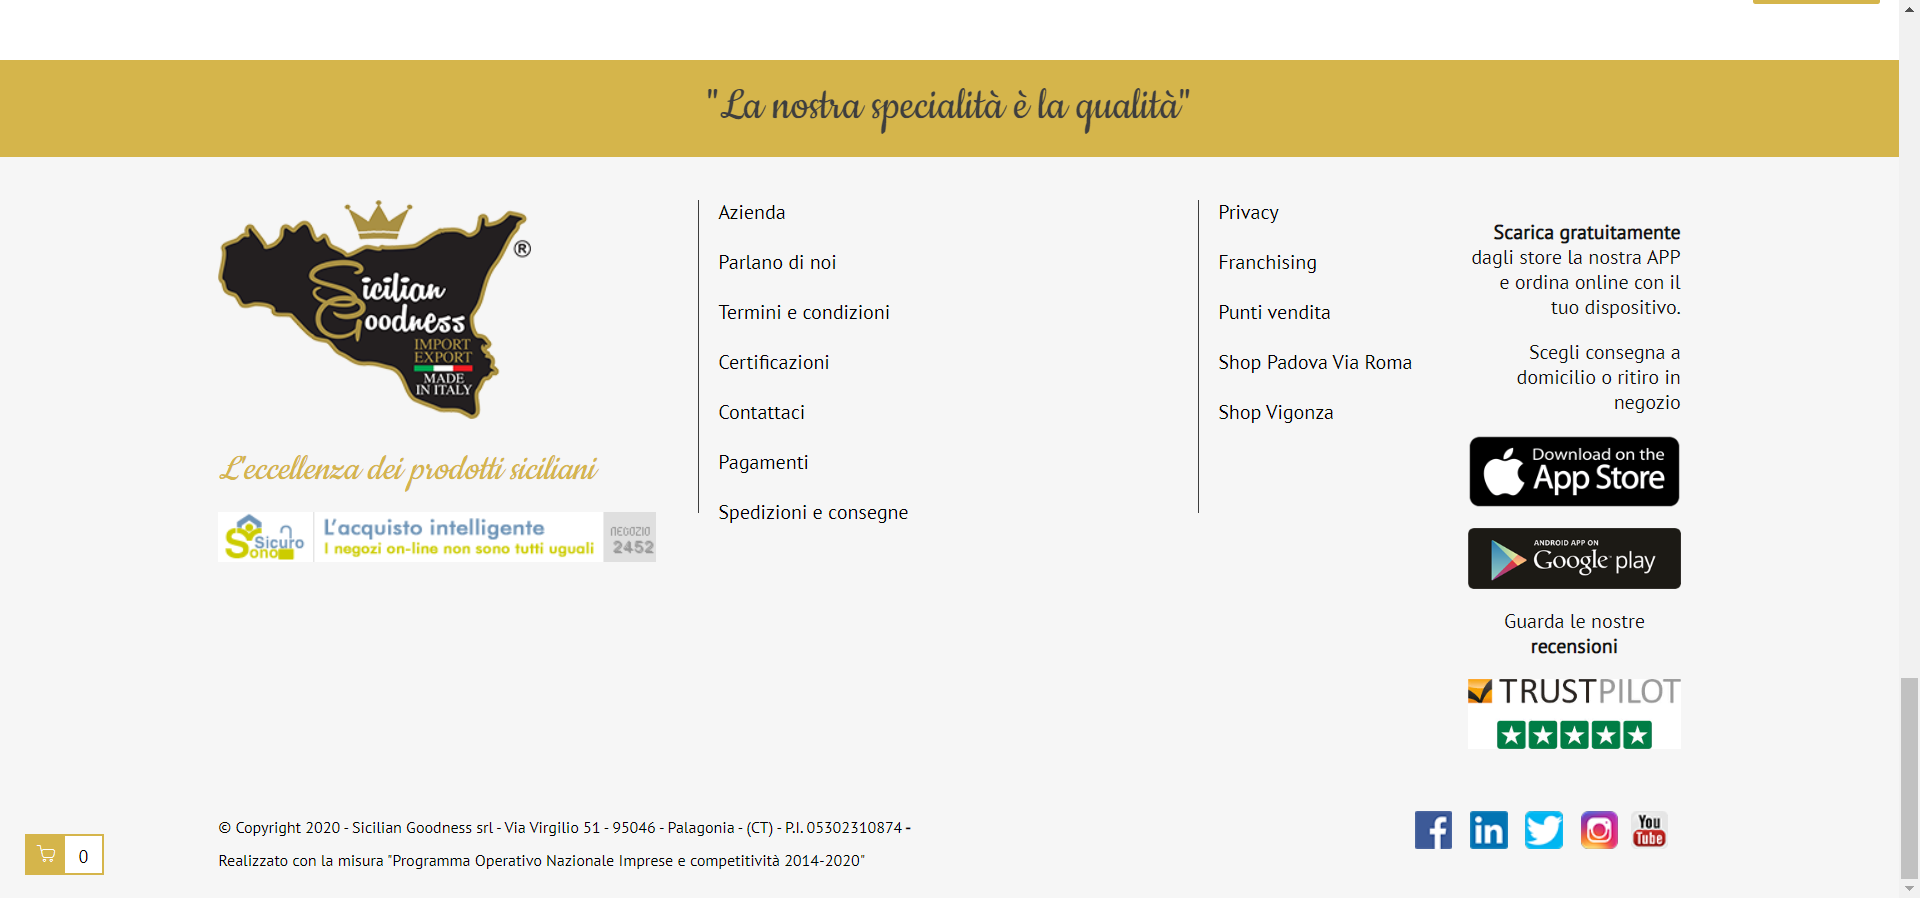
\includegraphics[width=12cm]{Img/contacts.png}
	\caption{Footer}
\end{figure}


\subsection{The Six Ws}
The best way to evaluate the impact of the homepage is to analyze the so-called "Six Ws".

\subsubsection{Where?}

Question: \textit{Where did I (user) arrive?}
\newline
A user who arrives on the site for the first time immediately understands that it is on a site connected to the kitchen. Name and logo help the user to understand where he is. Indeed the user immediately understands that he is on a site that offers Sicilian products. After seeing the pictures and reading the text, the user understands perfectly where he is.

\begin{figure}[H]
	\centering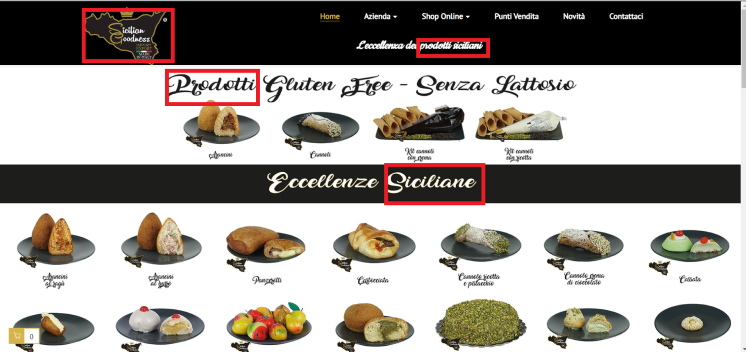
\includegraphics[width=12cm]{Img/where1.png}
	\caption{Where 1}
\end{figure}

\begin{figure}[H]
	\centering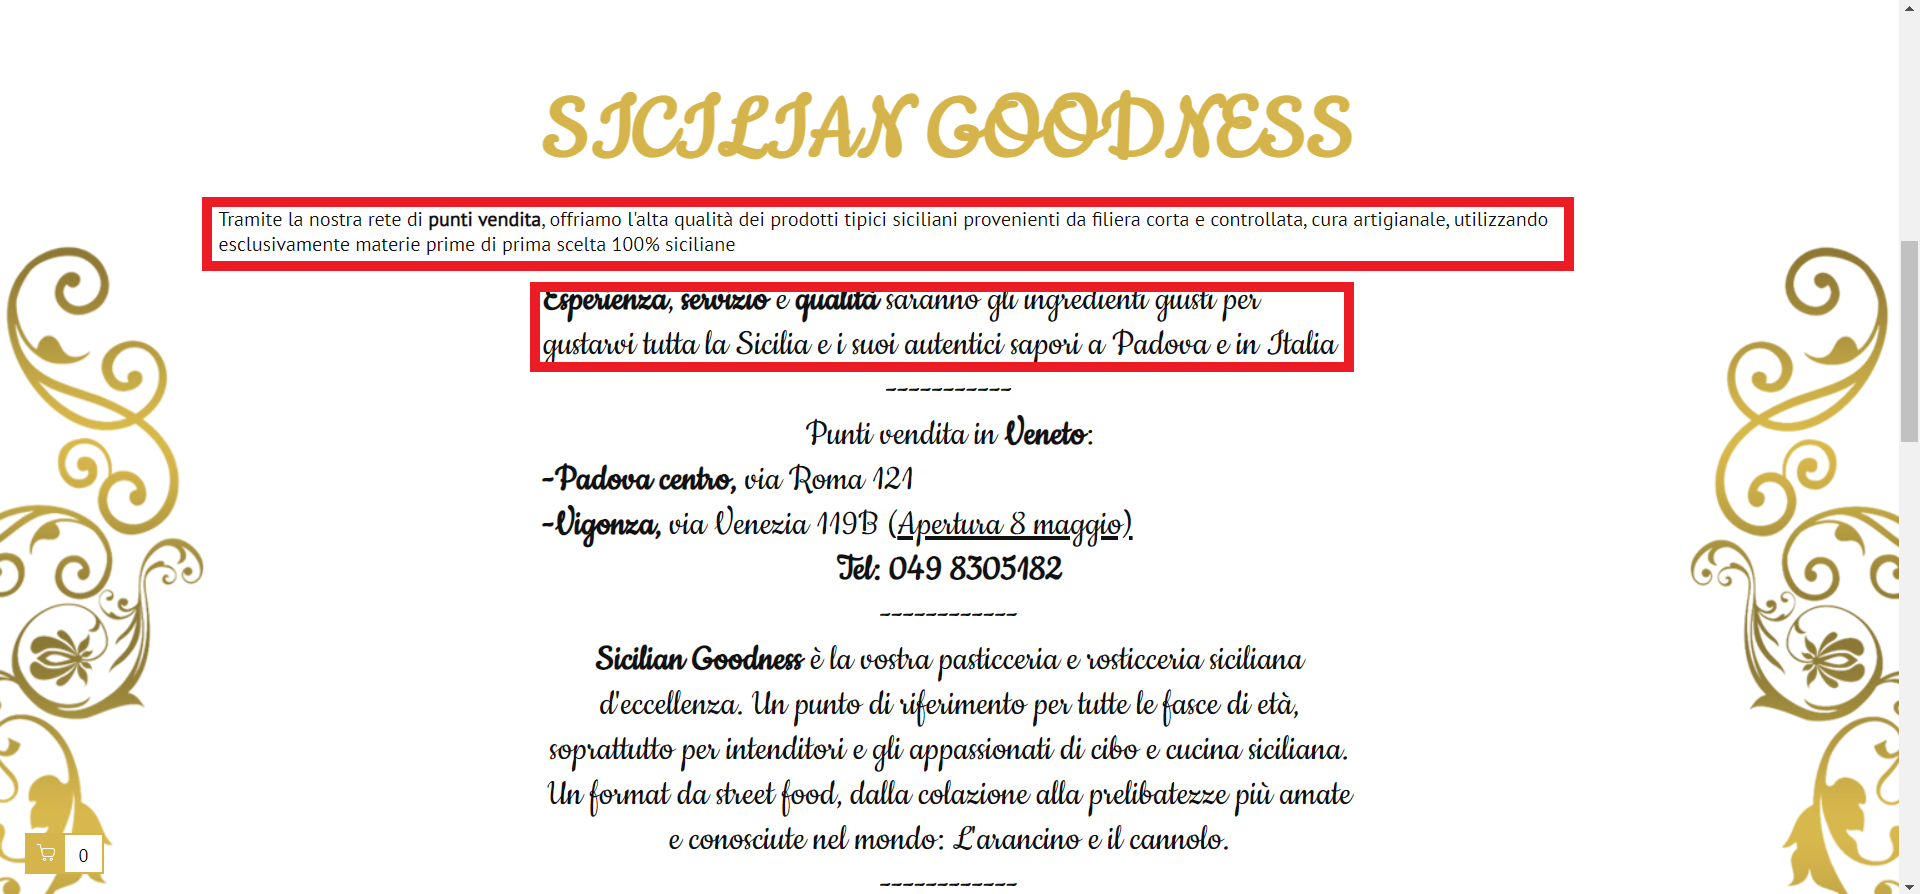
\includegraphics[width=12cm]{Img/where2.png}
	\caption{Where 2}
\end{figure}

\pagebreak

\subsubsection{Who?}

Question: \textit{Who is behind the website?}
\newline
The identity of the creator/owner of the site is not totally clear. Certainly the logo helps to identify it if you already know it, however for a user who has never heard of the site, the author is unknown and probably it will remain so. Indeed, to find some information about it, it is necessary scroll to the bottom of the page, until
to arrive in the footer, where the owner is written in a very small font, Sicilian Goodness srl. In addition, 'Azienda' and 'Parlano di noi' are two links that point to a page that offers some additional information about the company.
An other way is to click on 'Azienda' and 'Contattaci' in the top of the homepage. For these reasons, the Who axis is not well specified, as it takes too long to find an answer, which the user does not have and which can lead to increase dissatisfaction.

\begin{figure}[H]
	\centering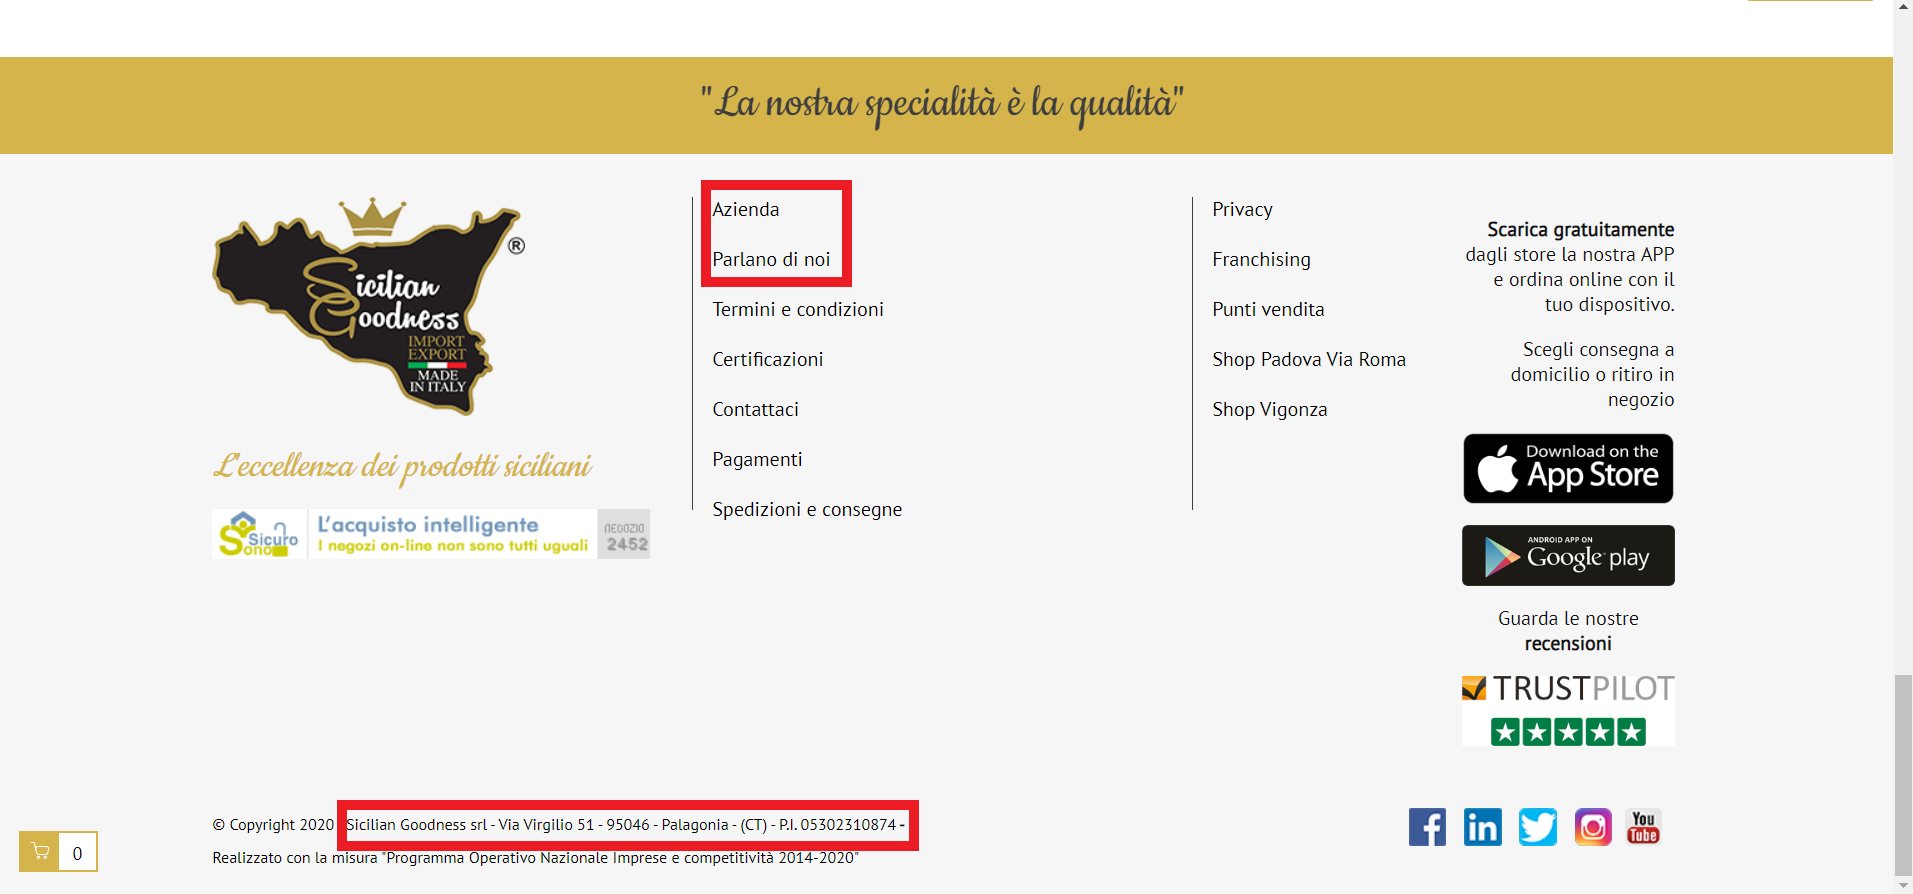
\includegraphics[width=12cm]{Img/who.png}
	\caption{Who}
\end{figure}

\subsubsection{Why?}

Question: \textit{What are the benefits? Why should I stay?}
\newline
The site specify very well why the user should stay in the website. In fact, the word 'Eccelenze' is repeated multiple times in the homepage.
In addition, as we can see in the image below, the site provide a short description to persuade the user to stay.
\begin{figure}[H]
	\centering
\includegraphics[width=12cm]{Img/why.png}
	\caption{Why}
\end{figure}

\pagebreak

\subsubsection{What?}

Question: \textit{What choices do I have?}
\newline
As before, the homepage is strongly oriented towards the content, which is proposed several times and in different ways. The main navigation menu presents several items that recall what the site offers. We understand immediately that this is an e-commerce to buy or order products online.

\subsubsection{When?}

Question: \textit{What are the last news?}
\newline
The When axis is clearly specified. Indeed in the navigation menu we have the section 'Novità'.
In addition, as we can see in the image below, the website offers in the homepage an appropriate section for the news.

\begin{figure}[H]
	\centering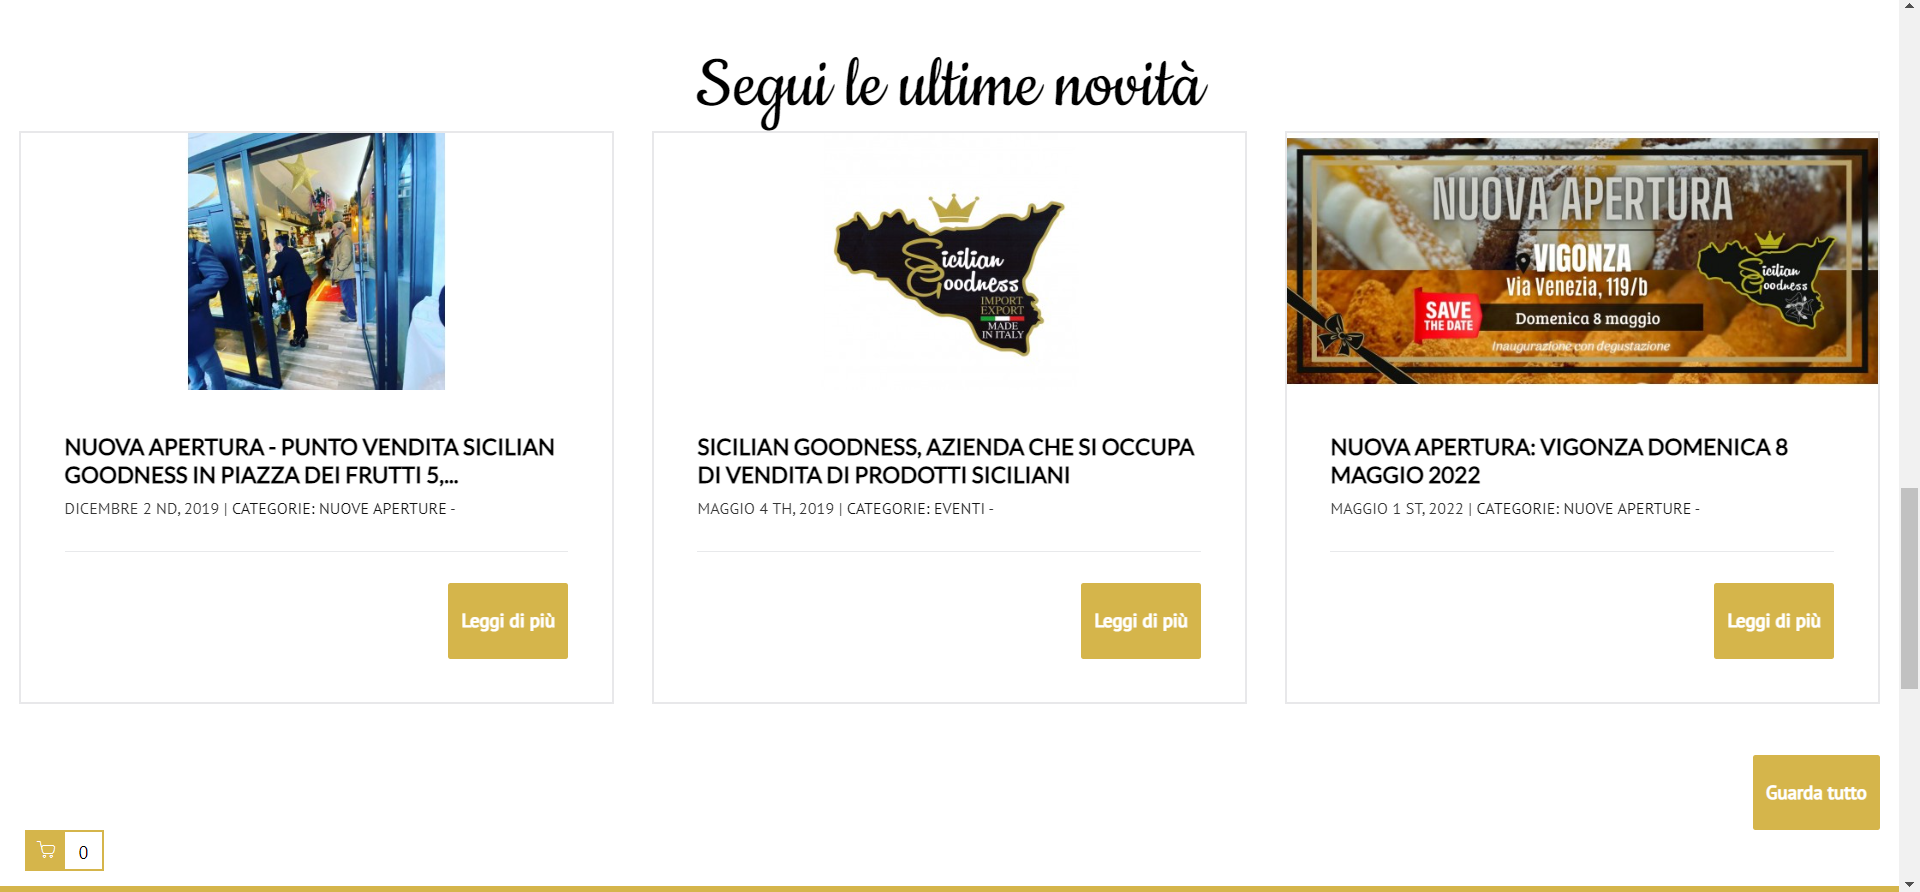
\includegraphics[width=12cm]{Img/news.png}
	\caption{When}
\end{figure}

\subsubsection{How?}

Question: \textit{How do I arrive where I want?}
\newline
The homepage offers a navigation menu to reach the pages that the user wants. The main menu is well specified in the top of the page.

\begin{figure}[H]
	\centering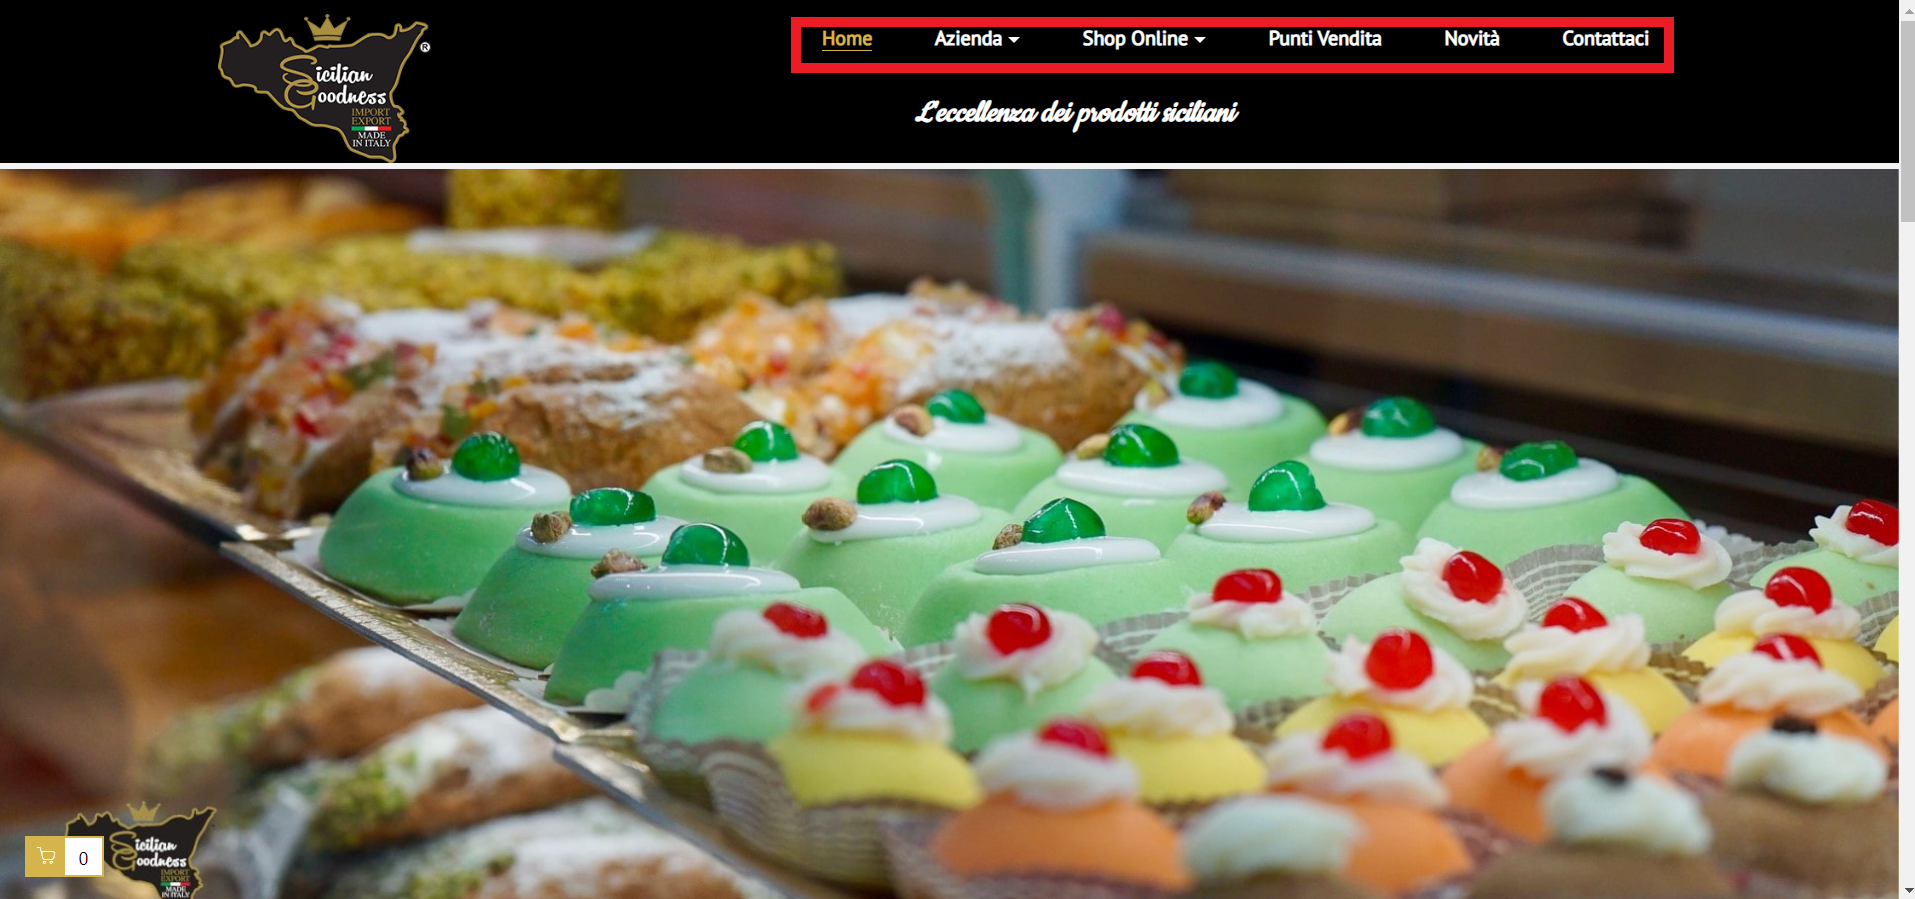
\includegraphics[width=12cm]{Img/how.png}
	\caption{How}
\end{figure}

\paragraph{Menu}
The menu presents the following items: 
\begin{itemize}
	\item Home: It's a link that reloads the website and it point to the homepage;
	\item Azienda: The underlying menu points to various pages that describe the company;
	\item Shop Online: The underlying menu points to the page where you can see the products and buy them;
	\item Punti Vendita: It points to a page that gives a description of the stores of the company, how to reach them and some useful information;
	\item Novità: It points to a page that provide all the news of the company;
	\item Contattaci: It points to a page with the contacts of the company.
\end{itemize}

\begin{figure}[H]
	\centering
\includegraphics[width=12cm]{Img/menu.png}
	\caption{Menu 1}
\end{figure}

The voice 'Azienda' offers the following items:
\begin{itemize}
	\item Chi siamo: It provides a description of the company and how it has evolved over time;
	\item Qualità: It provides a description of the quality of the products and how they are processed;
	\item Franchising: It provides a description about the franchising.
\end{itemize}

\begin{figure}[H]
	\centering
\includegraphics[width=12cm]{Img/menu2.png}
	\caption{Menu 2}
\end{figure}

The voice 'Shop Online' offers the following items:
\begin{itemize}
	\item SHOP VIGONZA: It points to the page where you can search the product that you want. This is an important page, because is what the user wants when it come in the site. In this page you can search, order and buy the products available in the shop of Vigonza;
	\item SHOP PADOVA VIA ROMA: It has the same functionality of the previous button(SHOP VIGONZA) but in this page you see only the products available in the other shop(Padova, Via Roma).
\end{itemize}

\begin{figure}[H]
	\centering
\includegraphics[width=12cm]{Img/menu3.png}
	\caption{Menu 3}
\end{figure}

\pagebreak